\chapter{振子、佔據數與第一個量子場}

量子場論是描述幾乎所有已知非重力物理的框架。這並不表示每個問題都能求解。氫原子尚可處理；到了硼這類原子，計算就已經困難得多；至於人體，則遠遠超出任何實際可行的場論計算能力。這個框架或許是基本的，但其中的方程仍然極其難解。

因此，我們將以最基本的方式開始。這個主題有時稱為\emph{二次量子化}，但在建立起所需的數學工具之前，這個名稱還不容易理解。最直接的途徑不是從相對論性場開始，而是從諧振子開始。重點不在彈簧，而在升降算符的代數。當這套代數推廣到許多模式時，升算符就不再只是``將振子提升一個能階''，而是真正具有``產生粒子''的意義。

\section{以代數描述振子}

對單一振子，令\(a^\dagger\)提高激發數，令\(a\)降低激發數。記號\(a_+\)與\(a_-\)等價，但匕首記號預示了場論中使用的語言。基態滿足
\begin{equation}
a|0\rangle=0,
\end{equation}
數算符則為
\begin{equation}
N=a^\dagger a,
\qquad
N|n\rangle=n|n\rangle.
\end{equation}
這兩個階梯算符互為厄米共軛，而其關鍵對易關係是
\begin{equation}
[a,a^\dagger]=1.
\label{eq:l06-single-commutator}
\end{equation}
這個簡單的代數幾乎涵蓋了振子的全部內容。

我們可以從位置與動量的適當線性組合得到\(a\)和\(a^\dagger\)。具體的約定取決於\(x\)、\(p\)、\(m\)和\(\omega\)的正規化；此處有用而不依賴約定的說法是，\(a^\dagger a\)可以重構二次振子的哈密頓量，但會少掉加上的基態能量。因此
\begin{equation}
H=\hbar\omega\left(N+\frac12\right).
\end{equation}
在目前的討論中，我們略去常數項，改用
\begin{equation}
H=\hbar\omega N.
\label{eq:l06-one-oscillator-hamiltonian}
\end{equation}
頻率決定每增加一個激發所需的能量。將\(n\)提高一個激發，需要\(\hbar\omega\)；將\(n\)降低一個激發，則會釋出相同的能量。

\section{多個互相獨立的振子}

現在考慮多個振子，並以\(i\)標記它們。這個標記只是指標，不是虛數單位。模式的數目可以有限，也可以無限。一組互相獨立的彈簧是一種圖像；理想小提琴弦的簡正模式則是另一種。在場論的應用中，重要的是無限多個模式的情形。

獨立性也有算符上的意義。真正屬於互相獨立子系統的算符彼此對易。若不對易，相應的物理量就不能獨立測量，而這些系統也就不是互相獨立的。因此
\begin{align}
[a_i,a_j]&=0, \\
[a_i^\dagger,a_j^\dagger]&=0, \\
[a_i,a_j^\dagger]&=\delta_{ij}.
\label{eq:l06-many-commutators}
\end{align}
當\(i\ne j\)時，屬於這兩個模式的所有量都彼此對易。當\(i=j\)時，最後一行就化為式~\eqref{eq:l06-single-commutator}。

每個振子都有自己的數算符，通常也有自己的頻率：
\begin{equation}
N_i=a_i^\dagger a_i,
\qquad
H=\sum_i\hbar\omega_i N_i.
\label{eq:l06-many-hamiltonian}
\end{equation}
共同本徵態以完整的一組數值標記：
\begin{equation}
|n_1,n_2,n_3,\ldots\rangle,
\qquad n_i=0,1,2,\ldots.
\label{eq:l06-occupation-ket}
\end{equation}
整數\(n_i\)稱為第\(i\)個振子的\emph{佔據數}。此刻這還只是名稱；不久之後，它就會用來計數佔據某個單粒子態的粒子，這個名稱也將名副其實。

所有佔據數都為零的態是
\begin{equation}
|0\rangle\equiv|0,0,0,\ldots\rangle,
\qquad a_i|0\rangle=0\quad\text{for every }i.
\label{eq:l06-oscillator-vacuum}
\end{equation}

\begin{classroomqa}
\lecturetimestamp{00:15:27}
\audiencequestion{無限多個振子是否對應到小提琴弦這類系統的連續模式？}
\lecturerresponse{理想化的弦是如此。真實的弦由原子構成，因此波長短到一定程度時，最終會遇到微觀尺度的截斷。不過，連續模型仍能啟發場論中使用的無限多個模式。}
\end{classroomqa}

\section{階梯係數為何是平方根}

\(a^\dagger\)的作用必須將\(N\)的一個本徵態升至下一個本徵態，但正規化條件仍容許一個係數：
\begin{equation}
a^\dagger|n\rangle=c_n|n+1\rangle.
\label{eq:l06-unknown-coefficient}
\end{equation}

\begin{figure}[htbp]
\centering
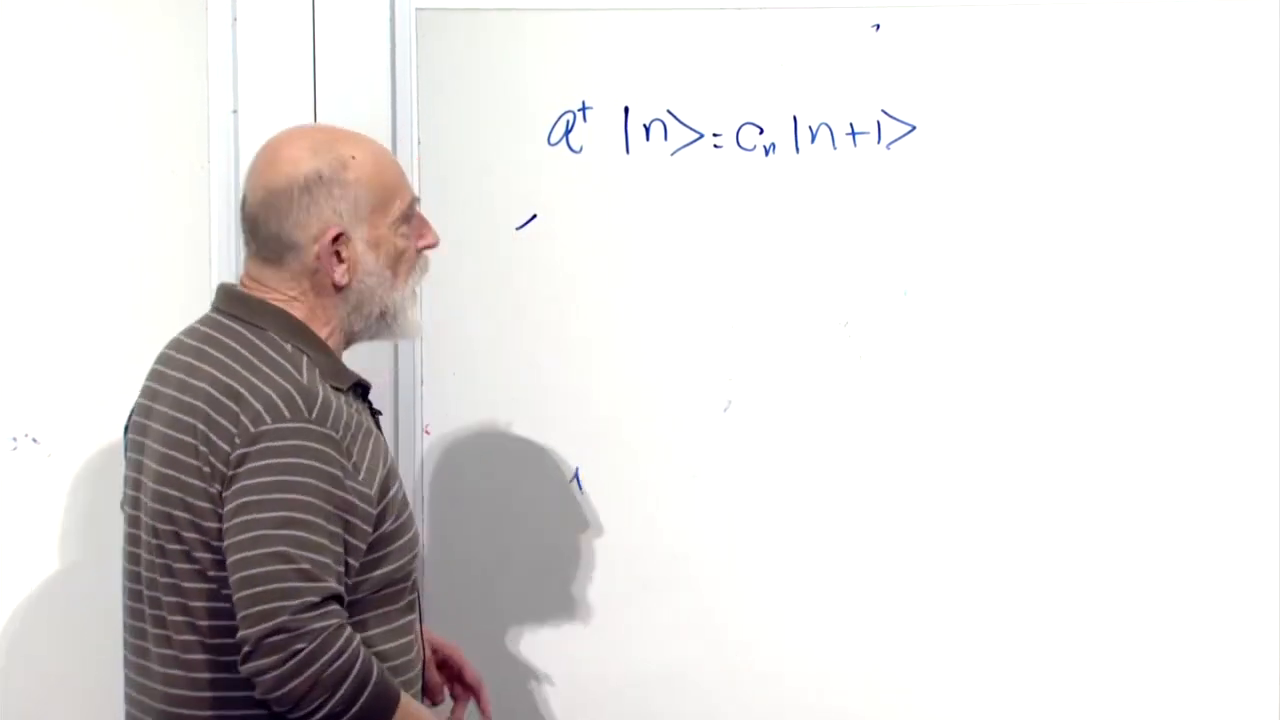
\includegraphics[width=0.9\linewidth]{lecture_06_frame_01.png}
\caption{階梯係數先被引入，之後才推導其正規化。黑板上的方程重現於式~\eqref{eq:l06-unknown-coefficient}。}
\lectureframe{00:19:38}
\end{figure}

選定相位慣例，使\(c_n\)為實數。取厄米共軛可得
\begin{equation}
\langle n|a=c_n\langle n+1|.
\end{equation}
將兩個關係相乘，並利用基底態已正規化的條件，
\begin{align}
c_n^2
&=\langle n|aa^\dagger|n\rangle \\
&=\langle n|(a^\dagger a+1)|n\rangle \\
&=\langle n|(N+1)|n\rangle \\
&=n+1.
\end{align}
因此，
\begin{equation}
a^\dagger|n\rangle=\sqrt{n+1}\,|n+1\rangle.
\label{eq:l06-raising-rule}
\end{equation}

\begin{classroomqa}
\lecturetimestamp{00:22:35}
\audiencequestion{求出\(c_n\)之前，為什麼可以先令\(\langle n+1|n+1\rangle=1\)？}
\lecturerresponse{本徵向量從一開始就選為正規化的基底。它們的正規化並不能決定\(a^\dagger|n\rangle\)的正規化；尚未確定的部分正是係數\(c_n\)。}
\end{classroomqa}

降階規則也可用相同方法推得：
\begin{equation}
a|n\rangle=\sqrt n\,|n-1\rangle.
\label{eq:l06-lowering-rule}
\end{equation}
當\(n=0\)時，係數會自動變為零，因此此規則也包含\(a|0\rangle=0\)。對多個模式而言，算符只會改變自身所對應位置上的佔據數：
\begin{align}
a_i^\dagger|n_1,\ldots,n_i,\ldots\rangle
&=\sqrt{n_i+1}\,|n_1,\ldots,n_i+1,\ldots\rangle, \\
a_i|n_1,\ldots,n_i,\ldots\rangle
&=\sqrt{n_i}\,|n_1,\ldots,n_i-1,\ldots\rangle.
\label{eq:l06-multimode-ladders}
\end{align}
其他項目都不會改變。

\section{波函數不是量子場}

定義場之前，必須先將它與熟悉的波函數區分開來。三個對比有助於理解這個轉變。

第一，單粒子波函數
\begin{equation}
\psi(x)=\langle x|\psi\rangle
\end{equation}
是態向量的一種表示，本身並不是可觀測量。我們測量的是位置、動量、角動量等算符；波函數提供振幅，據此可以計算各種測量結果的機率。

第二，多粒子波函數取決於所有粒子的位置。對兩個粒子，暫且將它們的位置向量稱為\(x\)和\(y\)，則
\begin{equation}
\psi(x,y)=\langle x,y|\psi\rangle.
\end{equation}
這裡的\(x\)和\(y\)代表兩個不同粒子的位置；它們不是同一個位置向量的笛卡兒\(x\)分量與\(y\)分量。對\(N\)個粒子而言，態由下式表示：
\begin{equation}
\psi(x_1,x_2,\ldots,x_N).
\end{equation}

第三，這個波函數描述的是粒子數固定的系統。十五粒子的波函數有十五個位置變數，屬於十五粒子希爾伯特空間。它本身無法描述粒子數從十五變成十四或十六的過程。

量子場則具有相反的特徵：它是算符而非態，依賴單一空間點\(x\)，並作用於涵蓋所有粒子數扇區的態空間。「``一個點''」是指一個可自由變動的位置向量，並不是說\(x\)已被指定為某個數值。

有一項限制在後面會很重要。以下引入的場\(\Psi(x)\)並非厄米算符，因此嚴格來說，它本身不是可觀測量。它的厄米組合才是可觀測量。因此，先前暫時說場可測量，現在要進一步精確說明，而不是撤回：場是算符值函數，而它們的厄米組合代表可測量的物理量。

\begin{classroomqa}
\lecturetimestamp{00:36:52}
\audiencequestion{如果場是位置的函數，位置可以變動嗎？雙粒子波函數中的\(y\)又到哪裡去了？}
\lecturerresponse{點\(x\)會在整個空間中變動。``一個位置''是指算符只有一個空間變數，不是說這個變數固定不動。在\(\psi(x,y)\)中，符號\(x\)和\(y\)分別表示兩個粒子的位置；等價地說，它們是\(x_1\)和\(x_2\)。它們不是場的變數的兩個笛卡兒分量。}
\end{classroomqa}

\begin{classroomqa}
\lecturetimestamp{00:38:15}
\audiencequestion{粒子數固定的波函數描述與場描述如何關聯？它們描述的是不同種類的粒子嗎？}
\lecturerresponse{兩者之間的關聯，正是接下來要建立的核心架構。這些粒子屬於同一種類。本講討論的是玻色子；費米子則需要不同的代數。}
\end{classroomqa}

\section{盒中的單粒子}

暫時回到普通的單粒子量子力學。將一個粒子放進一維盒中。只有一個粒子時，玻色子與費米子的差異無關緊要：沒有第二個相同粒子可用來檢驗交換或排他效應。

令
\begin{equation}
\psi_1(x),\ \psi_2(x),\ \psi_3(x),\ldots
\end{equation}
為能量本徵函數。最低模式是最平滑、且在盒壁處為零的波。下一個模式有一個內部節點；能量更高的模式則振盪得更快。對於寬度為\(L\)的理想無限深方形位能井，一組方便的正規化基底為
\begin{equation}
\psi_i(x)=\sqrt{\frac{2}{L}}\sin\!\left(\frac{i\pi x}{L}\right),
\qquad 0<x<L.
\label{eq:l06-box-basis}
\end{equation}
這個明確的正弦公式是黑板上定性草圖的一種標準表示方式；以下論證只需要一組完備且正交正規的單粒子態。

\begin{figure}[htbp]
\centering
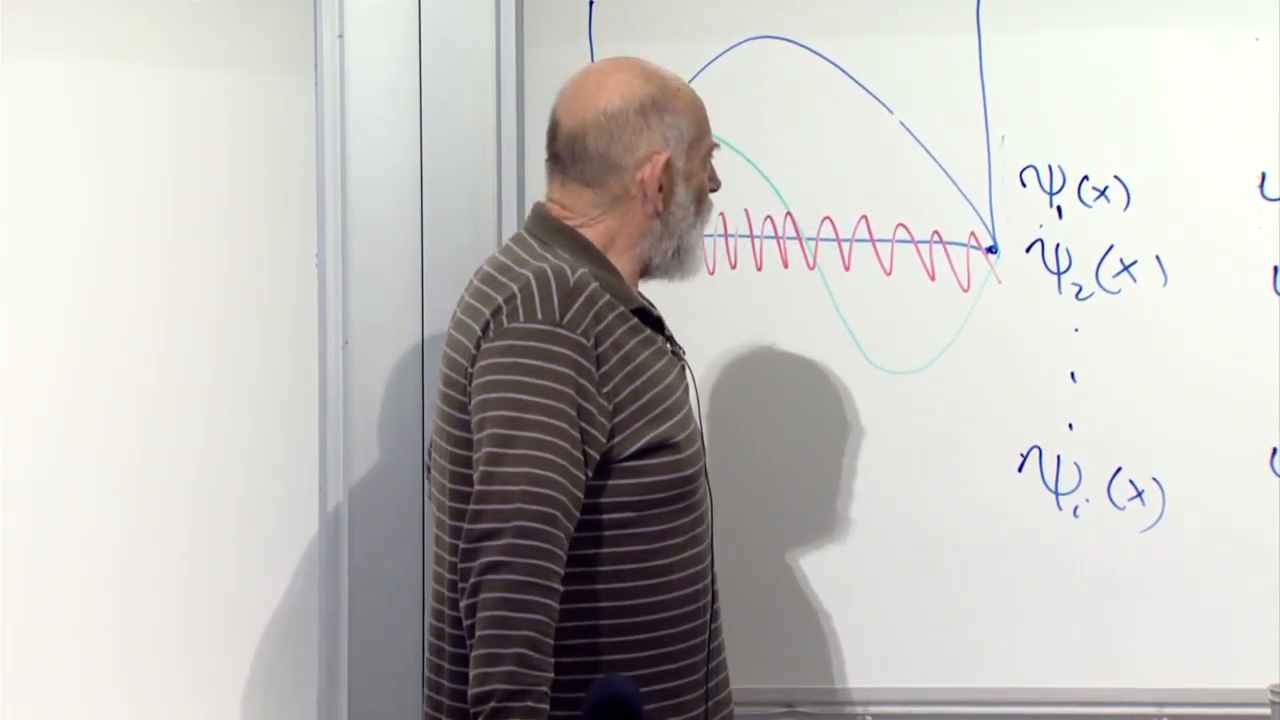
\includegraphics[width=0.9\linewidth]{lecture_06_frame_03.png}
\caption{依能量遞增排列的單粒子盒中模式。第一個模式沒有內部節點，第二個有一個；未畫出的高階模式則振盪得愈來愈快。}
\lectureframe{00:43:10}
\end{figure}

同樣的結構也可以重新繪製，避免受到現場黑板內容遮擋：
\begin{figure}[htbp]
\centering
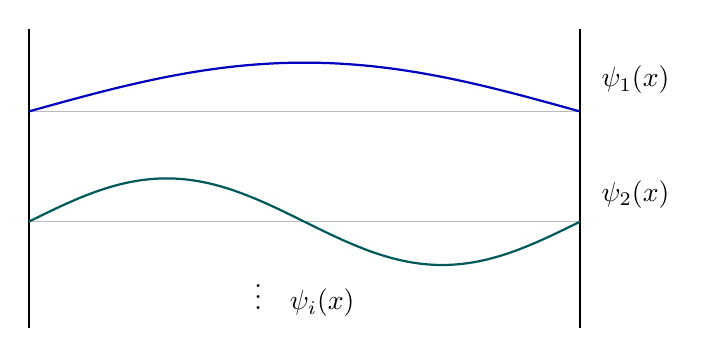
\begin{tikzpicture}[x=1cm,y=1cm]
  \draw[thick] (0,0) -- (0,3.8);
  \draw[thick] (7,0) -- (7,3.8);
  \draw[gray!55] (0,2.75) -- (7,2.75);
  \draw[gray!55] (0,1.35) -- (7,1.35);
  \draw[blue!75!black,thick,domain=0:7,samples=120]
    plot (\x,{2.75+0.62*sin(180*\x/7)});
  \draw[teal!70!black,thick,domain=0:7,samples=120]
    plot (\x,{1.35+0.55*sin(360*\x/7)});
  \node[right] at (7.15,3.15) {$\psi_1(x)$};
  \node[right] at (7.15,1.70) {$\psi_2(x)$};
  \node at (3.5,0.45) {$\vdots\quad \psi_i(x)$};
\end{tikzpicture}
\caption{盒中模式定性草圖的清晰重繪。為便於辨識，本徵函數在垂直方向上錯開；這不是額外的物理座標。}
\end{figure}

指標\(i\)標記的是單粒子態，不是粒子，也不是節點數。對盒中的基底而言，\(i\)恰好比內部節點數多一。每個態都有能量\(\varepsilon_i\)。依照講課時使用的記號，可以將這個能量寫成\(\hbar\omega_i\)；令\(\hbar=1\)後，也可以簡寫為\(\omega_i\)。

\begin{classroomqa}
\lecturetimestamp{00:39:01}
\audiencequestion{先前假設的獨立性是精確的嗎？指標\(i\)可以標記原子中電子的可能態嗎？}
\lecturerresponse{在獨立模式的架構中，不同模式之間的對易關係是精確的。這個指標可以用來標記原子的單粒子態。不過，若粒子之間有相互作用，簡單的獨立模式哈密頓量就無法完整描述系統。}
\end{classroomqa}

\begin{classroomqa}
\lecturetimestamp{00:40:34}
\audiencequestion{盒中的粒子是玻色子嗎？}
\lecturerresponse{可以是；但只有一個粒子時，統計性質並不重要。只有存在多個相同粒子時，排他效應與交換才有意義。}
\end{classroomqa}

\section{從盒中模式到福克空間}

現在允許盒中有任意數目的相同玻色子。數目為\(n_1\)的粒子可以佔據\(\psi_1\)，數目為\(n_2\)的粒子可以佔據\(\psi_2\)，依此類推。因此，一個基底態為
\begin{equation}
|n_1,n_2,n_3,\ldots\rangle.
\end{equation}
這正是我們用來描述多個振子的記號。兩者在結構上完全對應：每個單粒子態對應一個振子，而振子的激發數等於佔據該態的粒子數。

玻色子在此不可或缺，因為每個\(n_i\)都可以是任意非負整數。費米子的每個單粒子態則只能為空或被一個粒子佔據，不能有兩個粒子同時佔據，因此不能直接沿用一般的振子代數。

現在可以根據算符對佔據數基底的作用來定義這些算符。\(a_i^\dagger\)在單粒子態\(i\)中產生一個粒子；\(a_i\)則移除一個粒子：
\begin{align}
a_i^\dagger|n_1,\ldots,n_i,\ldots\rangle
&=\sqrt{n_i+1}\,|n_1,\ldots,n_i+1,\ldots\rangle, \\
a_i|n_1,\ldots,n_i,\ldots\rangle
&=\sqrt{n_i}\,|n_1,\ldots,n_i-1,\ldots\rangle.
\end{align}
這並非事後才作的類比，而是玻色子產生與湮滅算符在此基底上的定義。由於這組基底張成整個空間，透過線性延伸，這些定義就決定了算符對所有態的作用。

\begin{classroomqa}
\lecturetimestamp{00:47:11}
\audiencequestion{\(n_1,n_2,n_3\)是量子態嗎？}
\lecturerresponse{標記\(1,2,3,\ldots\)指出單粒子態；符號\(n_1,n_2,n_3,\ldots\)表示佔據這些態的粒子數。必須區分態的標記與其佔據數，這是此處主要的記號難點。}
\end{classroomqa}

\subsection{平方根的作用}

因子\(\sqrt{n_i+1}\)不代表額外粒子，也不代表另一種物理過程。它讓算符具有正確的正規化與代數性質。對單一模式而言，
\begin{align}
a a^\dagger|n\rangle
&=a\bigl(\sqrt{n+1}\,|n+1\rangle\bigr) \\
&=(n+1)|n\rangle,
\end{align}
而
\begin{equation}
a^\dagger a|n\rangle=n|n\rangle.
\end{equation}
兩者的差因此是\(|n\rangle\)，符合\([a,a^\dagger]=1\)的要求。非常粗略地說，兩個階梯算符各自的量級約為\(\sqrt n\)，因為它們的乘積會給出量級為\(n\)的數算符。

\begin{classroomqa}
\lecturetimestamp{00:47:52}
\audiencequestion{平方根因子有什麼具體的物理意義？}
\lecturerresponse{它主要是數學上的正規化因子，確保佔據態已正規化、\(a^\dagger a\)的本徵值為\(n\)，並確保階梯算符滿足振子的對易關係。有時候，數學本身就是所需的物理意義。}
\end{classroomqa}

\begin{classroomqa}
\lecturetimestamp{00:52:25}
\audiencequestion{產生算符和湮滅算符是否只根據它們的性質及對基底的作用來定義？}
\lecturerresponse{是的。定義不必建立在更基本的圖像之上。定義的價值要由其推論來檢驗。規定算符對一組完備基底的作用，就能定義它們對所有態的作用，而這些定義也會導出所需的對易關係。}
\end{classroomqa}

\begin{classroomqa}
\lecturetimestamp{00:53:22}
\audiencequestion{為什麼\(a_i\)會讓粒子消失，而不是只把它移到另一個態？}
\lecturerresponse{因為\(a_i\)的定義就是降低態\(i\)的佔據數。有用的問題不是某個定義為什麼成立，而是它為什麼有用。它之所以有用，是因為發射與吸收都需要改變粒子數的算符：輻射發射時會產生光子，吸收時則會湮滅光子。}
\end{classroomqa}

所有佔據數態所張成的空間稱為\emph{福克空間}。其中包含真空、所有單粒子態、所有雙粒子態，依此類推，沒有固定的上限：
\begin{equation}
\mathcal F=\mathcal H_0\oplus\mathcal H_1\oplus\mathcal H_2\oplus\cdots.
\label{eq:l06-fock-space}
\end{equation}
直和記號清楚表明了普通的\(N\)粒子波函數無法表達之處：所有粒子數扇區都屬於同一個態空間。

\begin{classroomqa}
\lecturetimestamp{00:54:56}
\audiencequestion{在佔據數本徵向量上定義算符，就能決定它們對任意向量的作用嗎？接著是否可得振子的對易關係？}
\lecturerresponse{正是如此。佔據數向量構成一組基底，因此透過線性性質，這些定義可延伸至整個福克空間。在這組基底上作用，就能驗證玻色子的對易關係。每個單粒子態都對應一個振子，而振子的佔據數就是該態中的粒子數。}
\end{classroomqa}

\subsection{真空與自由哈密頓量}

福克真空是所有單粒子態都沒有粒子佔據的態：
\begin{equation}
|0\rangle=|0,0,0,\ldots\rangle,
\qquad a_i|0\rangle=0.
\end{equation}
這裡的\emph{基態}一詞可能造成誤解。最低的\emph{單粒子}態是模式\(i=1\)；福克真空中連這個模式也沒有粒子。若有粒子佔據最低模式，\(a_1\)就可以將它移除，使系統回到真空。

\begin{classroomqa}
\lecturetimestamp{00:56:19}
\audiencequestion{用佔據數來說，真空是什麼？最低的單粒子態有粒子佔據嗎？}
\lecturerresponse{真空的所有佔據數都為零，並且會被每個\(a_i\)湮滅。真空中最低的單粒子模式沒有粒子佔據。若有粒子佔據其中，其湮滅算符就能將該粒子移除。}
\end{classroomqa}

對於沒有相互作用的粒子，總能量是各部分能量的總和。若態\(i\)中的一個粒子具有能量\(\hbar\omega_i\)，則
\begin{align}
H
&=\sum_i \hbar\omega_i N_i \\
&=\sum_i \hbar\omega_i a_i^\dagger a_i.
\label{eq:l06-free-fock-hamiltonian}
\end{align}
這個式子有兩種等價的解讀。一種是對振子能量求和，每個單粒子態對應一個振子；另一種是對單粒子能量求和，並將每個能量乘以具有該能量的粒子數。

在場論記號中，\(a_i^\dagger\)通常稱為產生算符，\(a_i\)稱為湮滅算符。較早使用的\(a_+\)與\(a_-\)記號表達的是相同概念。

\section{場出現之前的釐清}

休息後的幾個問題，將新的振子記數方式與普通粒子在振子位能中運動的情形區分開來。

\begin{classroomqa}
\lecturetimestamp{01:06:09}
\audiencequestion{盒中粒子的能階並非等間距，那麼諧振子在哪裡？}
\lecturerresponse{單粒子能量\(\omega_i\)不必等間距。不過，對每個固定模式\(i\)而言，該模式中有零個、一個、兩個或三個互不作用粒子時，能量分別為\(0,\omega_i,2\omega_i,3\omega_i\)。這個佔據數階梯才是這裡所說的振子；它不同於將一個粒子放進諧振子位能中。}
\end{classroomqa}

\begin{classroomqa}
\lecturetimestamp{01:08:38}
\audiencequestion{這個架構與傅立葉分解有關嗎？}
\lecturerresponse{關係非常密切。若單粒子基底由動量模式組成，模式函數就是正弦、餘弦或複指數，而\(a_i\)就是傅立葉係數的量子類比。一般基底不一定由三角函數組成，但展開的邏輯相同。}
\end{classroomqa}

\begin{classroomqa}
\lecturetimestamp{01:09:07}
\audiencequestion{所有粒子的能量都相同嗎？這裡有納入相互作用嗎？}
\lecturerresponse{佔據同一單粒子態的粒子能量相同；處於不同態的粒子，能量通常不同。目前粒子是自由的，也就是彼此不相互作用。相互作用會加入位能項，因此哈密頓量就不再只是式~\eqref{eq:l06-free-fock-hamiltonian}中的可加總和。}
\end{classroomqa}

\begin{classroomqa}
\lecturetimestamp{01:10:26}
\audiencequestion{每個振子中的半個零點能量量子到哪裡去了？}
\lecturerresponse{它是哈密頓量中的加法常數。常數與所有算符對易，因此不會改變海森堡運動方程；一般非重力測量則取決於能量差。這個常數在某些特殊用途上可能很重要，但不影響此處正在建立的架構。}
\end{classroomqa}

自由理論已經是一種威力非凡的記數工具。它不只追蹤許多粒子，也能追蹤粒子態的改變，以及粒子的產生、消失，或總粒子數不同的各種疊加態。這些算符不只是記數符號，因為適當的厄米組合可以測量；不過，記數仍是有用的初步直覺。

\begin{classroomqa}
\lecturetimestamp{01:14:03}
\audiencequestion{場論與量子場論的歷史起源為何？}
\lecturerresponse{簡要來說，這段歷史始於法拉第對電場與磁場的物理圖像，以及馬克士威描述經典場的方程。普朗克研究熱輻射時引入能量量子；愛因斯坦則將量子化與電磁場本身及光量子連結起來。到了1920年代前後，海森堡、泡利，尤其是狄拉克，進一步協助建立現代的算符架構。紫外災難與輻射的量子描述，是早期幾個關鍵問題。這只是一個概略的歷史梗概，並未完整判定各項工作的優先權歸屬。}
\end{classroomqa}

這段歷史也說明了振子為何一再出現。腔中的經典輻射可以分解為簡正模式。將這些模式量子化後，其激發數就成了光子數。佔據模式的數學量子於是成為物理粒子。

\section{玻色場算符}

令\(\{\psi_i(x)\}\)為一組完備且正交正規的單粒子波函數基底。定義
\begin{equation}
\boxed{\Psi(x)=\sum_i a_i\,\psi_i(x)}
\label{eq:l06-field-annihilation}
\end{equation}
以及它的厄米共軛
\begin{equation}
\boxed{\Psi^\dagger(x)=\sum_i a_i^\dagger\,\psi_i^*(x)}.
\label{eq:l06-field-creation}
\end{equation}

\begin{figure}[htbp]
\centering
\includegraphics[width=0.9\linewidth]{lecture_06_frame_04.png}
\caption{湮滅場及其厄米共軛的完整模式展開。排版後的式子~\eqref{eq:l06-field-annihilation}和\eqref{eq:l06-field-creation}保留了相同的算符與複共軛結構。}
\lectureframe{01:25:15}
\end{figure}

對任意固定的位置\(x\)而言，每個\(\psi_i(x)\)都是普通的複數。所有算符成分都在\(a_i\)和\(a_i^\dagger\)之中。隨著\(x\)變動，空間中的每一點都對應不同的算符。這就是\(\Psi\)作為算符值函數的確切含義。

若基底函數是平面波，式~\eqref{eq:l06-field-annihilation}和\eqref{eq:l06-field-creation}就是量子版的傅立葉展開：經典傅立葉係數在此變成了算符。在盒中，基底也可以採用式~\eqref{eq:l06-box-basis}中的正弦函數。任何完備且正交正規的單粒子基底都適用。

\(\Psi\)和\(\Psi^\dagger\)都不是厄米算符。可觀測場可以由厄米組合構成，例如
\begin{equation}
\Psi(x)+\Psi^\dagger(x),
\qquad
i\bigl(\Psi^\dagger(x)-\Psi(x)\bigr),
\end{equation}
稍後也會以\(\Psi^\dagger(x)\Psi(x)\)這類乘積構造可觀測密度。目前首先要了解的是這兩個基本場的作用。

\begin{classroomqa}
\lecturetimestamp{01:23:14}
\audiencequestion{右邊的模式函數是普通波函數，左邊怎麼會是算符？}
\lecturerresponse{選定\(x\)後，函數\(\psi_i(x)\)就是數值。因子\(a_i\)是算符。數乘上算符仍是算符，因此總和也是算符。改變\(x\)，就會得到一整族算符。}
\end{classroomqa}

\section{場的作用}

湮滅場會立刻湮滅真空：
\begin{equation}
\Psi(x)|0\rangle
=\sum_i\psi_i(x)a_i|0\rangle
=0.
\label{eq:l06-field-kills-vacuum}
\end{equation}
產生場的作用則更能說明問題。

令\(|i\rangle\)表示波函數為
\begin{equation}
\langle x|i\rangle=\psi_i(x).
\end{equation}
的單粒子態。單粒子基底的完備性給出
\begin{equation}
\sum_i|i\rangle\langle i|=1.
\label{eq:l06-completeness}
\end{equation}
將此恆等式作用於位置本徵態：
\begin{align}
|x\rangle
&=\sum_i|i\rangle\langle i|x\rangle \\
&=\sum_i\psi_i^*(x)|i\rangle.
\label{eq:l06-position-expansion}
\end{align}
在福克空間的記號中，單粒子模式態為
\begin{equation}
|i\rangle=a_i^\dagger|0\rangle.
\end{equation}
將其代入式~\eqref{eq:l06-position-expansion}，可得
\begin{align}
|x\rangle
&=\sum_i\psi_i^*(x)a_i^\dagger|0\rangle \\
&=\Psi^\dagger(x)|0\rangle.
\label{eq:l06-local-creation}
\end{align}
因此，\(\Psi^\dagger(x)\)會在\(x\)處產生一個局域化粒子，而\(\Psi(x)\)則會在該處湮滅一個粒子。位置本徵態具有狄拉克 {\proseunicodefont δ} 函數的局域化性質，是一種廣義且不可正規化的態；實際的局域化粒子則須以可正規化的波包將場加權積分而得。\editorialnote{本講採用理想的位置本徵態描述。波包這項補充說明交代了標準的數學意義，並未改變論證。}

\begin{classroomqa}
\lecturetimestamp{01:36:26}
\audiencequestion{如何指定所產生粒子種類的資訊？在\(x\)處的態是狄拉克 {\proseunicodefont δ} 函數局域化的嗎？}
\lecturerresponse{每種粒子都對應一個獨立的場，因此粒子的種類由所使用的場決定。變數\(x\)指定粒子在哪裡產生。在理想的位置基底中，所產生的態具有狄拉克 {\proseunicodefont δ} 函數的局域化性質。}
\end{classroomqa}

玻色子種類的例子包括光子、重力子、希格斯玻色子與膠子，不過實際的場也帶有內部指標。即使是光子也需要偏振標記。簡化的純量場記號省略這些額外標記，讓粒子產生的原理更清楚。

\subsection{真空不是零向量}

方程
\begin{equation}
\Psi(x)|0\rangle=0
\end{equation}
中以零表示的兩個對象截然不同。右矢\(|0\rangle\)是真空，是一個正規化的物理態，滿足
\begin{equation}
\langle0|0\rangle=1.
\end{equation}
右側的結果則是零向量。它的範數為零，無法正規化，也不代表物理態。

做加法時，兩者的差異就很明顯。將零向量加到單粒子態上，結果不變；將真空加到單粒子態上，則會得到不同粒子數扇區的真正疊加態。使用正規化係數時，
\begin{equation}
|\chi\rangle=\frac{1}{\sqrt2}\bigl(|0\rangle+|1\rangle\bigr)
\end{equation}
零粒子與一個粒子的機率相同。這個態不同於\(|1\rangle\)。

\begin{classroomqa}
\lecturetimestamp{01:37:23}
\audiencequestion{如果在\(x\)處沒有粒子，\(\Psi(x)\)是否就什麼也不做？結果為零又代表什麼？}
\lecturerresponse{它不會返回原來的態，而是返回零向量。真空是描述空間為空的歸一化態；零向量的長度為零，且不描述任何物理態。任何算符作用在零向量上，都會返回零向量。}
\end{classroomqa}

\begin{classroomqa}
\lecturetimestamp{01:39:00}
\audiencequestion{如果把真空而非零向量加到單粒子態上，會得到什麼？}
\lecturerresponse{得到的是一個包含不同粒子數振幅的疊加態。相較之下，加上零向量不會改變單粒子態。符號\(|0\rangle\)表示零佔據數，並不代表零向量。}
\end{classroomqa}

\begin{classroomqa}
\lecturetimestamp{01:41:56}
\audiencequestion{在場的展開式中，模式函數與其產生或湮滅算符的次序重要嗎？模式函數可以是複數嗎？}
\lecturerresponse{模式函數是普通數，因此與所有算符對易，次序並不重要。一般而言，模式函數可以是複數；所選基底是實數還是複數，取決於單粒子Schr\"odinger問題。}
\end{classroomqa}

\subsection{兩粒子與玻色對稱性的形成}

要在\(x\)處產生一個粒子，並在\(y\)處產生另一個粒子，只要作用兩次：
\begin{equation}
|x,y\rangle
=\Psi^\dagger(y)\Psi^\dagger(x)|0\rangle.
\label{eq:l06-two-particle-state}
\end{equation}
這兩個位置可以重合，也可以不同。由於底層的產生算符彼此對易，
\begin{align}
[\Psi^\dagger(x),\Psi^\dagger(y)]
&=\sum_{i,j}\psi_i^*(x)\psi_j^*(y)
[a_i^\dagger,a_j^\dagger] \\
&=0.
\end{align}
因此可得
\begin{equation}
\Psi^\dagger(y)\Psi^\dagger(x)|0\rangle
=\Psi^\dagger(x)\Psi^\dagger(y)|0\rangle.
\label{eq:l06-boson-exchange}
\end{equation}
交換兩個粒子的次序不會造成任何改變，這正是玻色交換對稱性。因此，我們也可以從振子代數出發，\emph{推導出}由彼此對易的產生算符所構造的粒子是玻色子。費米子則需要使用反對易算符。

\begin{classroomqa}
\lecturetimestamp{01:42:37}
\audiencequestion{如何在單粒子態中加入第二個粒子？}
\lecturerresponse{再作用一個產生場即可。若要在\(y\)處加入粒子，就讓\(\Psi^\dagger(y)\)作用在\(\Psi^\dagger(x)\)的左側。所得結果就是方程式~\eqref{eq:l06-two-particle-state}中的兩粒子態。}
\end{classroomqa}

\begin{classroomqa}
\lecturetimestamp{01:46:04}
\audiencequestion{兩個產生場彼此對易，是否就完全等同於將兩粒子態對稱化？}
\lecturerresponse{是。這使得一個粒子在\(x\)處、另一個在\(y\)處的態，與交換標記後得到的態完全相同。這就是全同玻色子的定義性交換性質。}
\end{classroomqa}

\begin{classroomqa}
\lecturetimestamp{01:46:32}
\audiencequestion{這是否表示\(x\)和\(y\)處的粒子必須是同一種類的玻色子？}
\lecturerresponse{是。\(x\)和\(y\)是位置，而一個場描述一種粒子。不同種類的粒子，以及例如光子的兩種偏振等額外標記，都需要不同的場分量。}
\end{classroomqa}

\section{可變粒子數為何重要}

如果一個問題永遠都恰好包含三十七個粒子，那麼場的語言就只是可有可無的記帳方式。場論真正的威力，在粒子可以被發射和吸收時才會顯現；尤其當粒子數本身是量子變數時，更是如此。Fock 空間允許如下形式的態：
\begin{equation}
|\Phi\rangle
=c_0|0\rangle+c_1|1\rangle+c_2|2\rangle+\cdots,
\qquad
\sum_{n=0}^{\infty}|c_n|^2=1.
\end{equation}
雷射場是一個重要例子：它通常不是具有確定光子數的態，而是許多粒子數扇區的疊加。

粒子與場之間的橋樑如今已清楚呈現。模式算符計數能量本徵態中的粒子，並改變粒子數；場則將這些算符與一組完備波函數結合，使粒子能在指定位置被產生或移除。諧振子的代數已成為玻色量子場的基本語言。
